\vspace{1cm}
\subsection*{\underline{Solution}}
\[ \text{max } Z = 6x_1 + 8x_2\]  

\[    
\left\{
    \begin{array}{l}
        6x_{1} + 3x_{2} \leq 18 \\[2pt]
        2x_{1} + 3x_{2} \leq 9 \\[2pt]
        x_{1}, x_{2} \text{ are integers}
    \end{array}
    \right.
\]

\begin{center}
    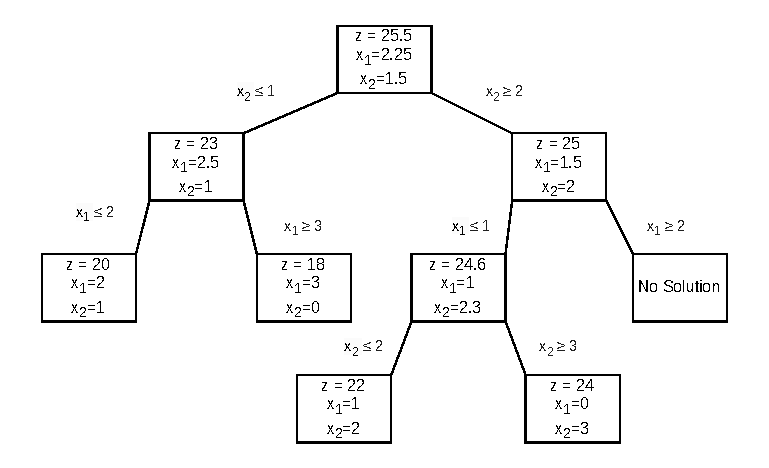
\includegraphics{Exercice/PY/EX1/b1.drawio.pdf}
\end{center}

\vspace{0.5cm}

\[\text{Optimal Solution is }\hspace{0.1cm} \boxed{(x_1,x_2) = (0,3)}\]

\begin{center}
    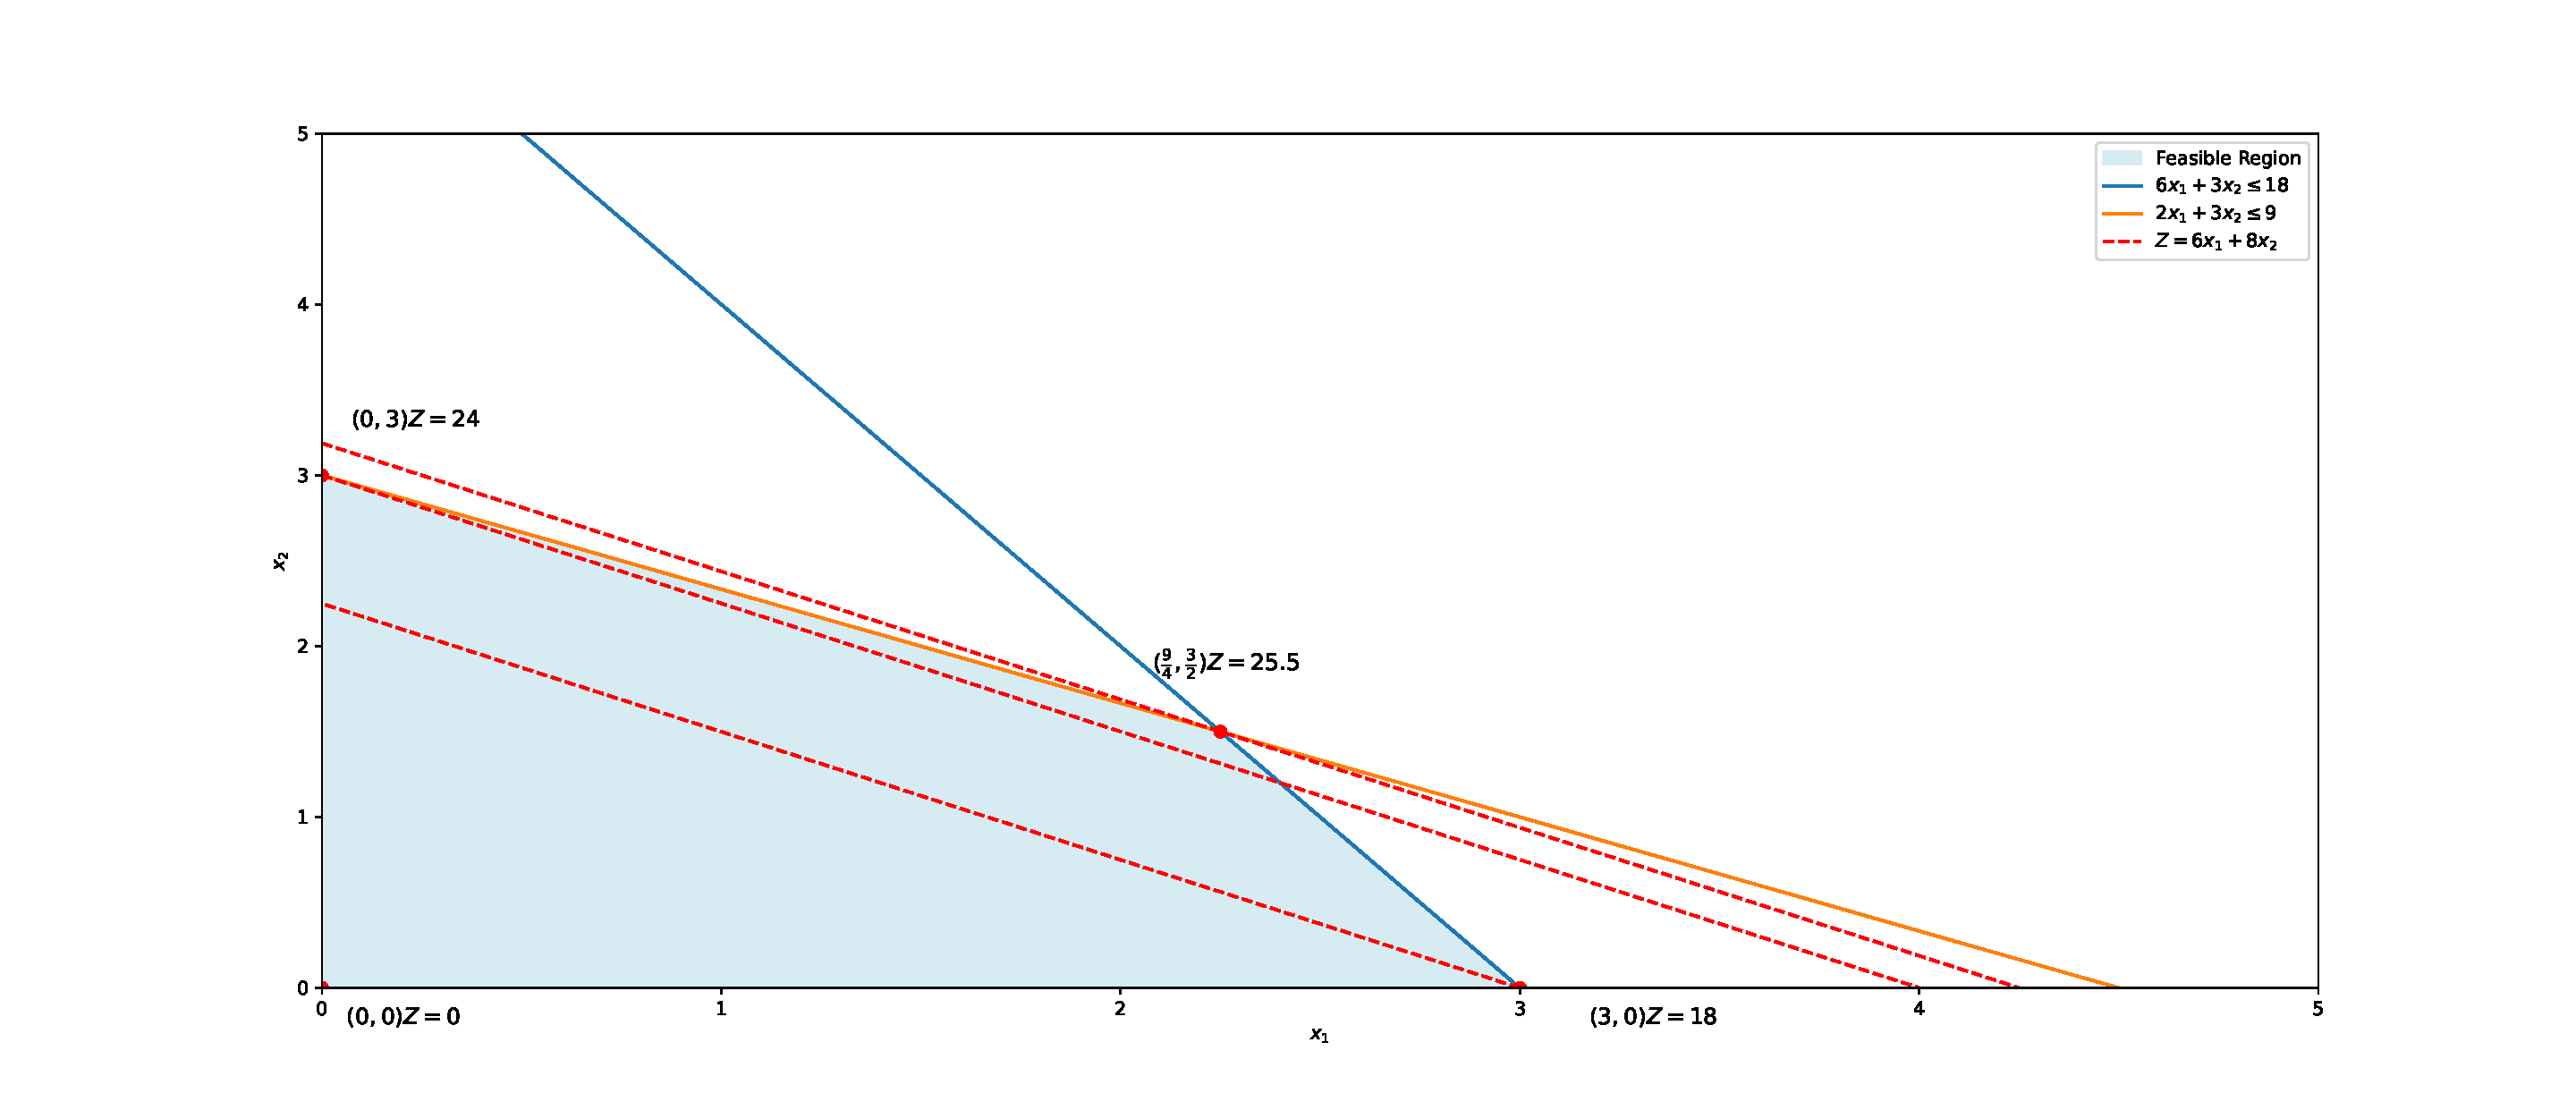
\includegraphics[width = \textwidth]{Exercice/PY/EX1/ex1.1.pdf}
\end{center}


\begin{center}
    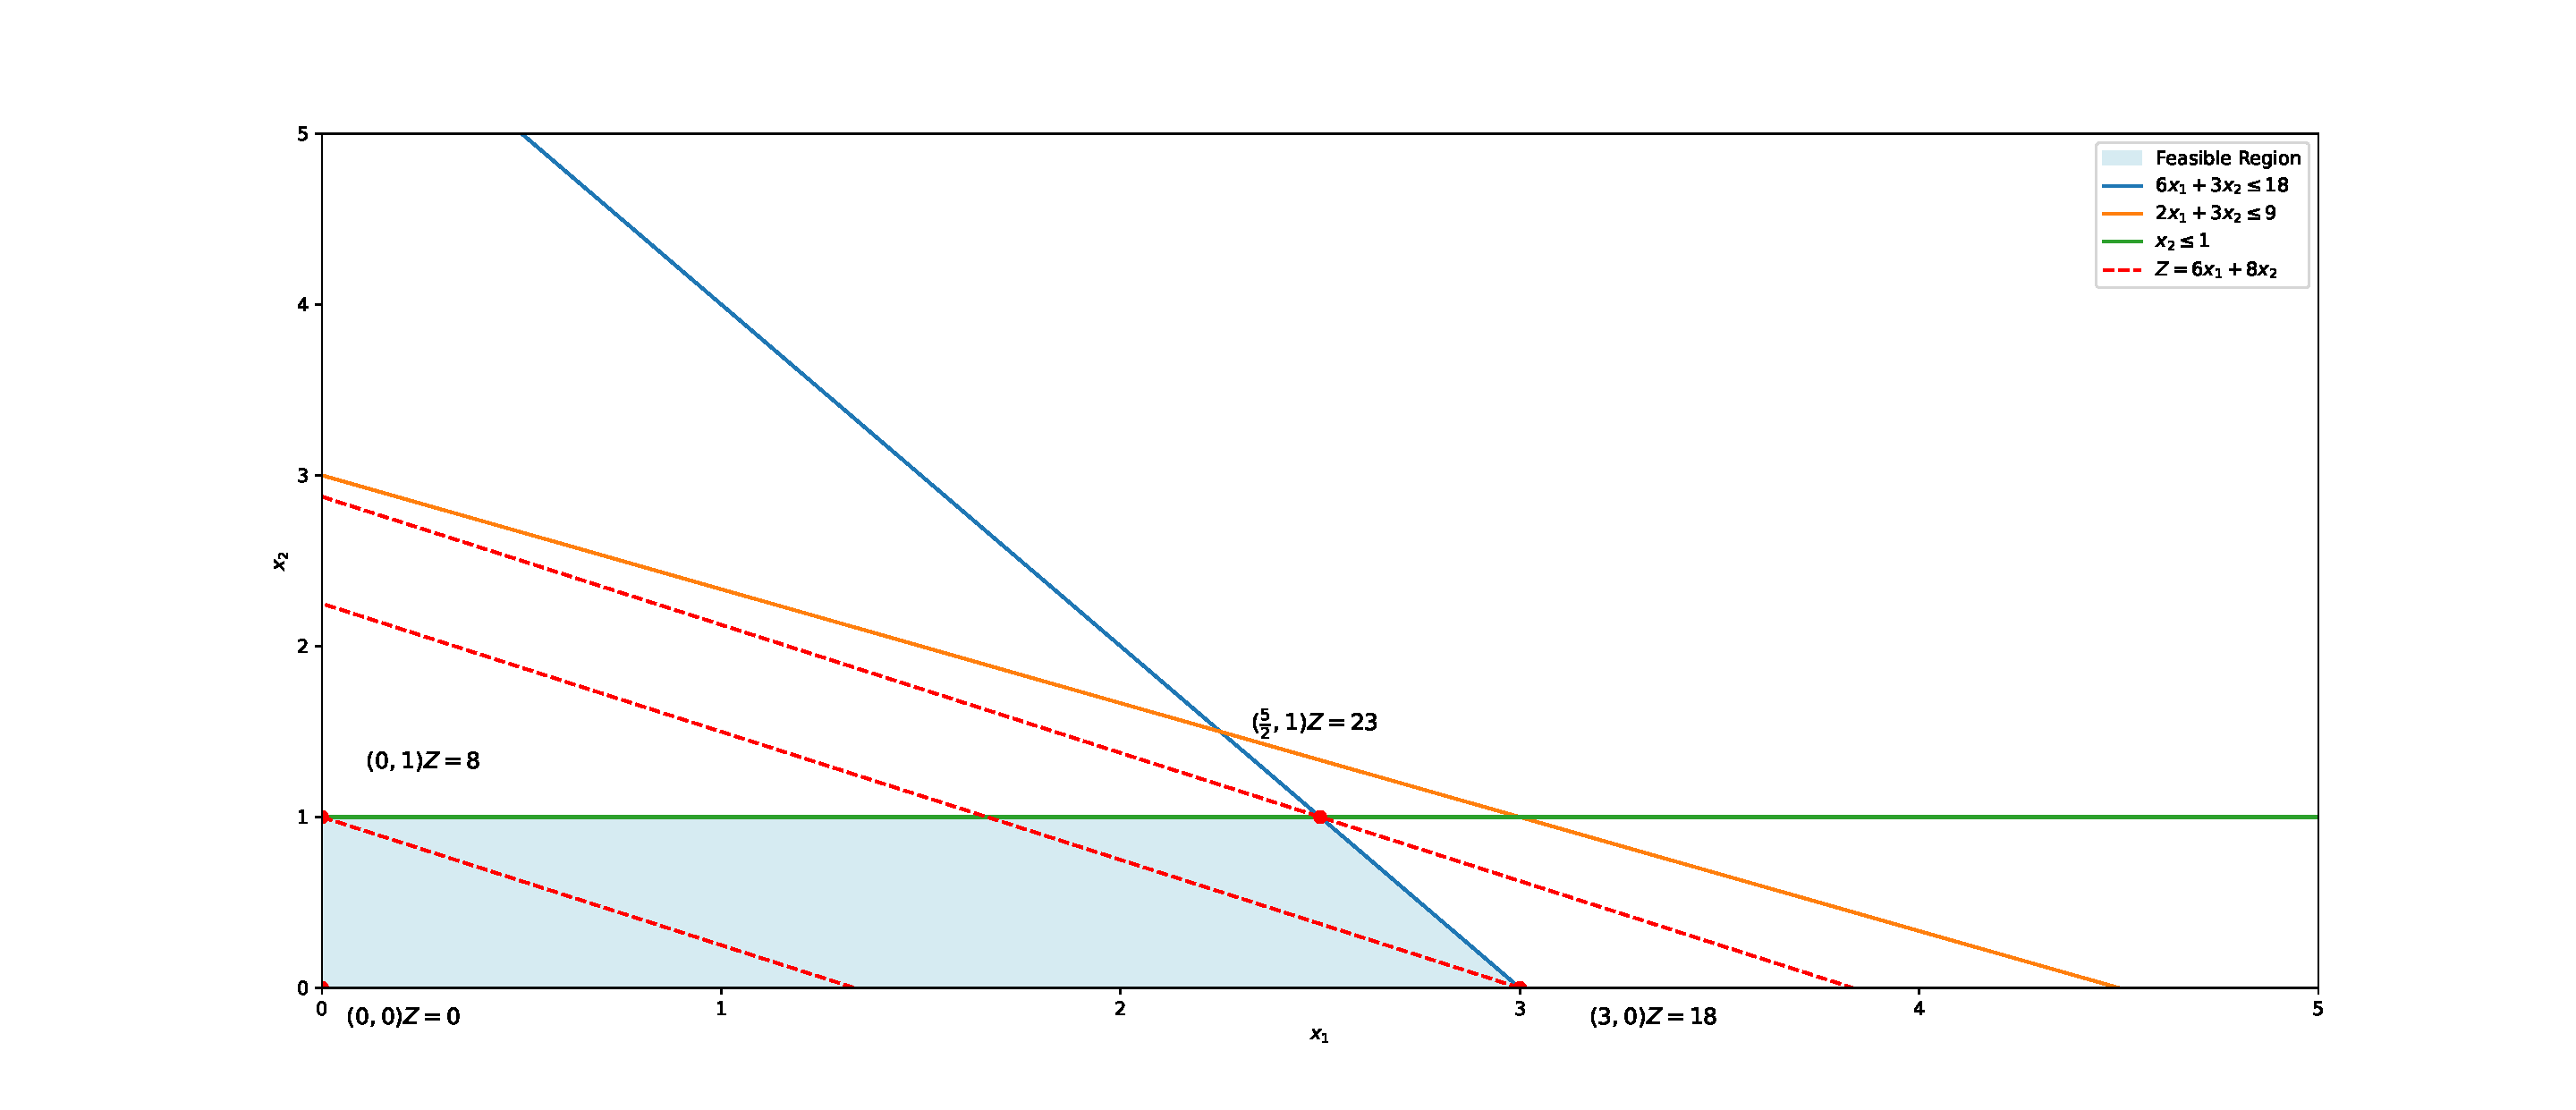
\includegraphics[width = \textwidth]{Exercice/PY/EX1/ex1.2.pdf}
\end{center}


\begin{center}
    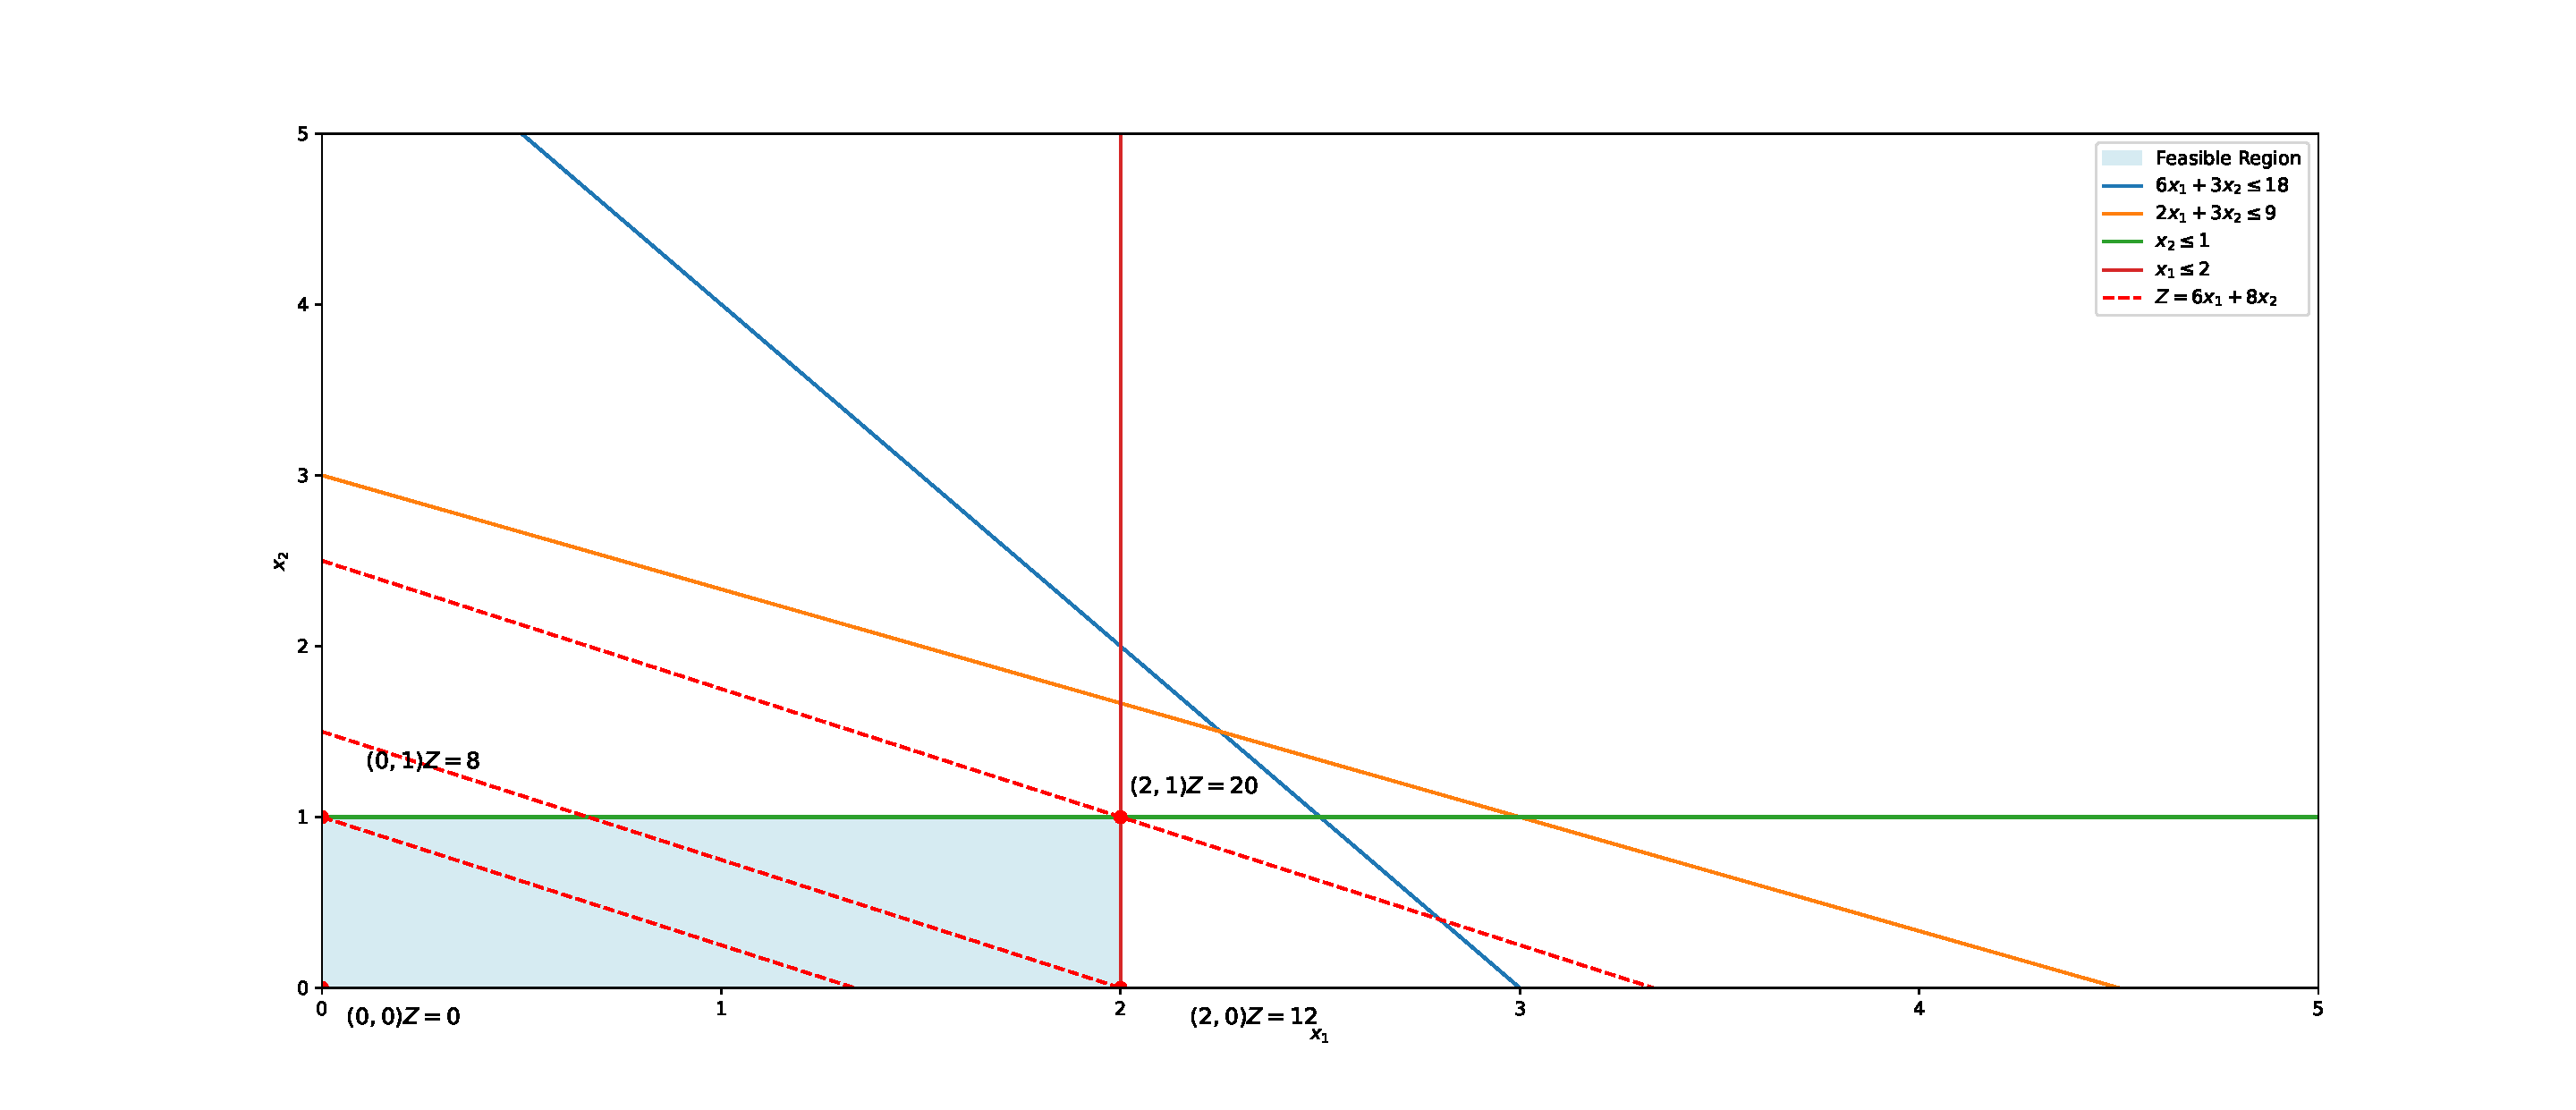
\includegraphics[width = \textwidth]{Exercice/PY/EX1/ex1.3.pdf}
\end{center}

\begin{center}
    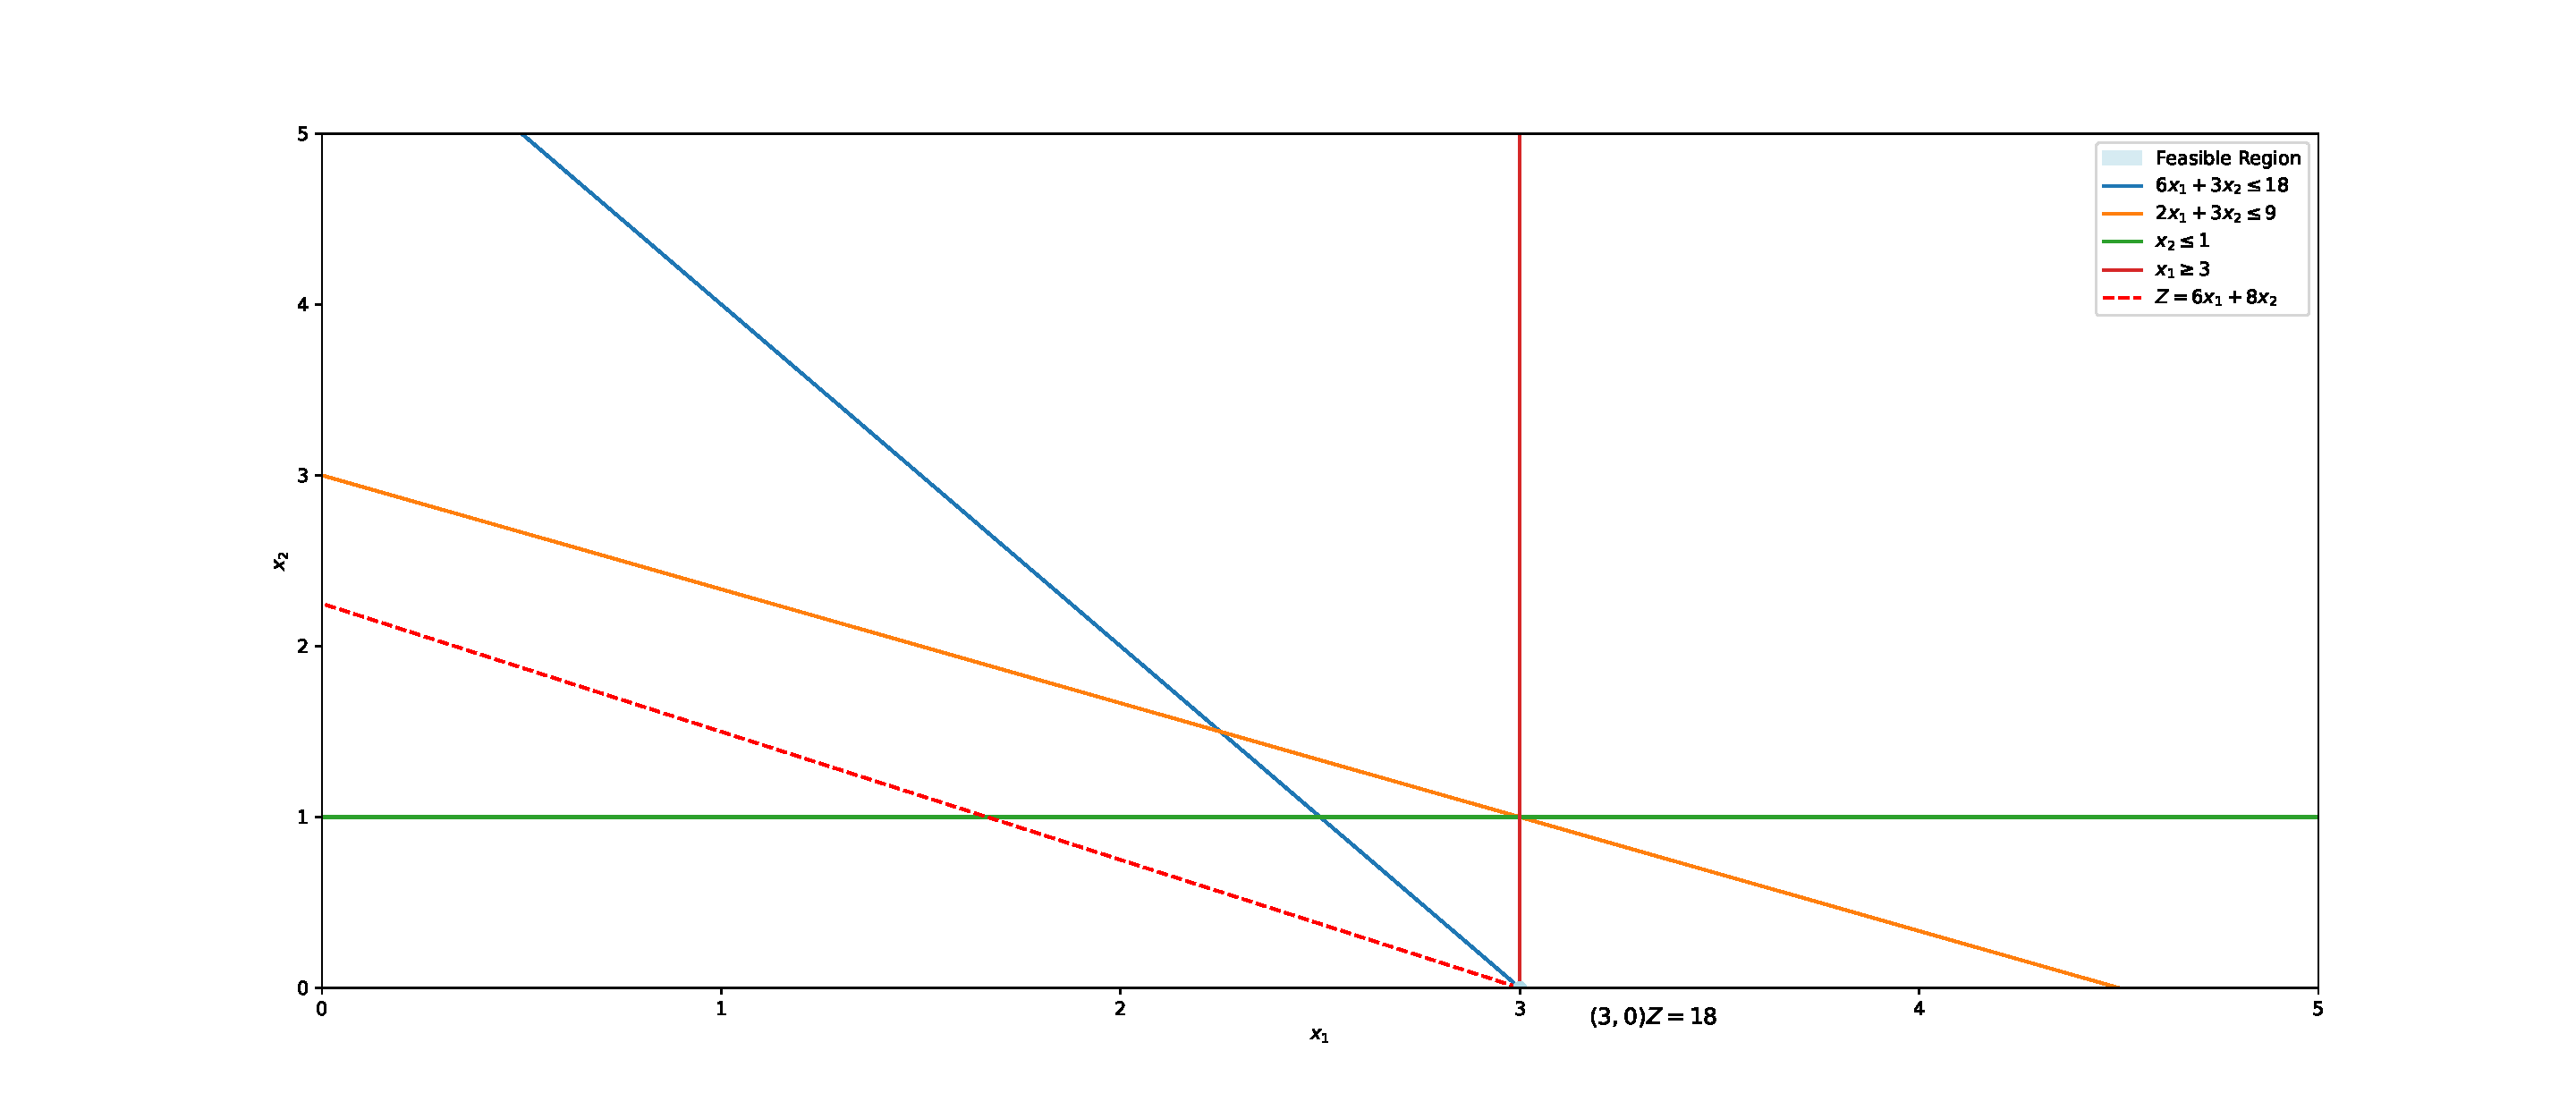
\includegraphics[width = \textwidth]{Exercice/PY/EX1/ex1.4.pdf}
\end{center}
\begin{center}
    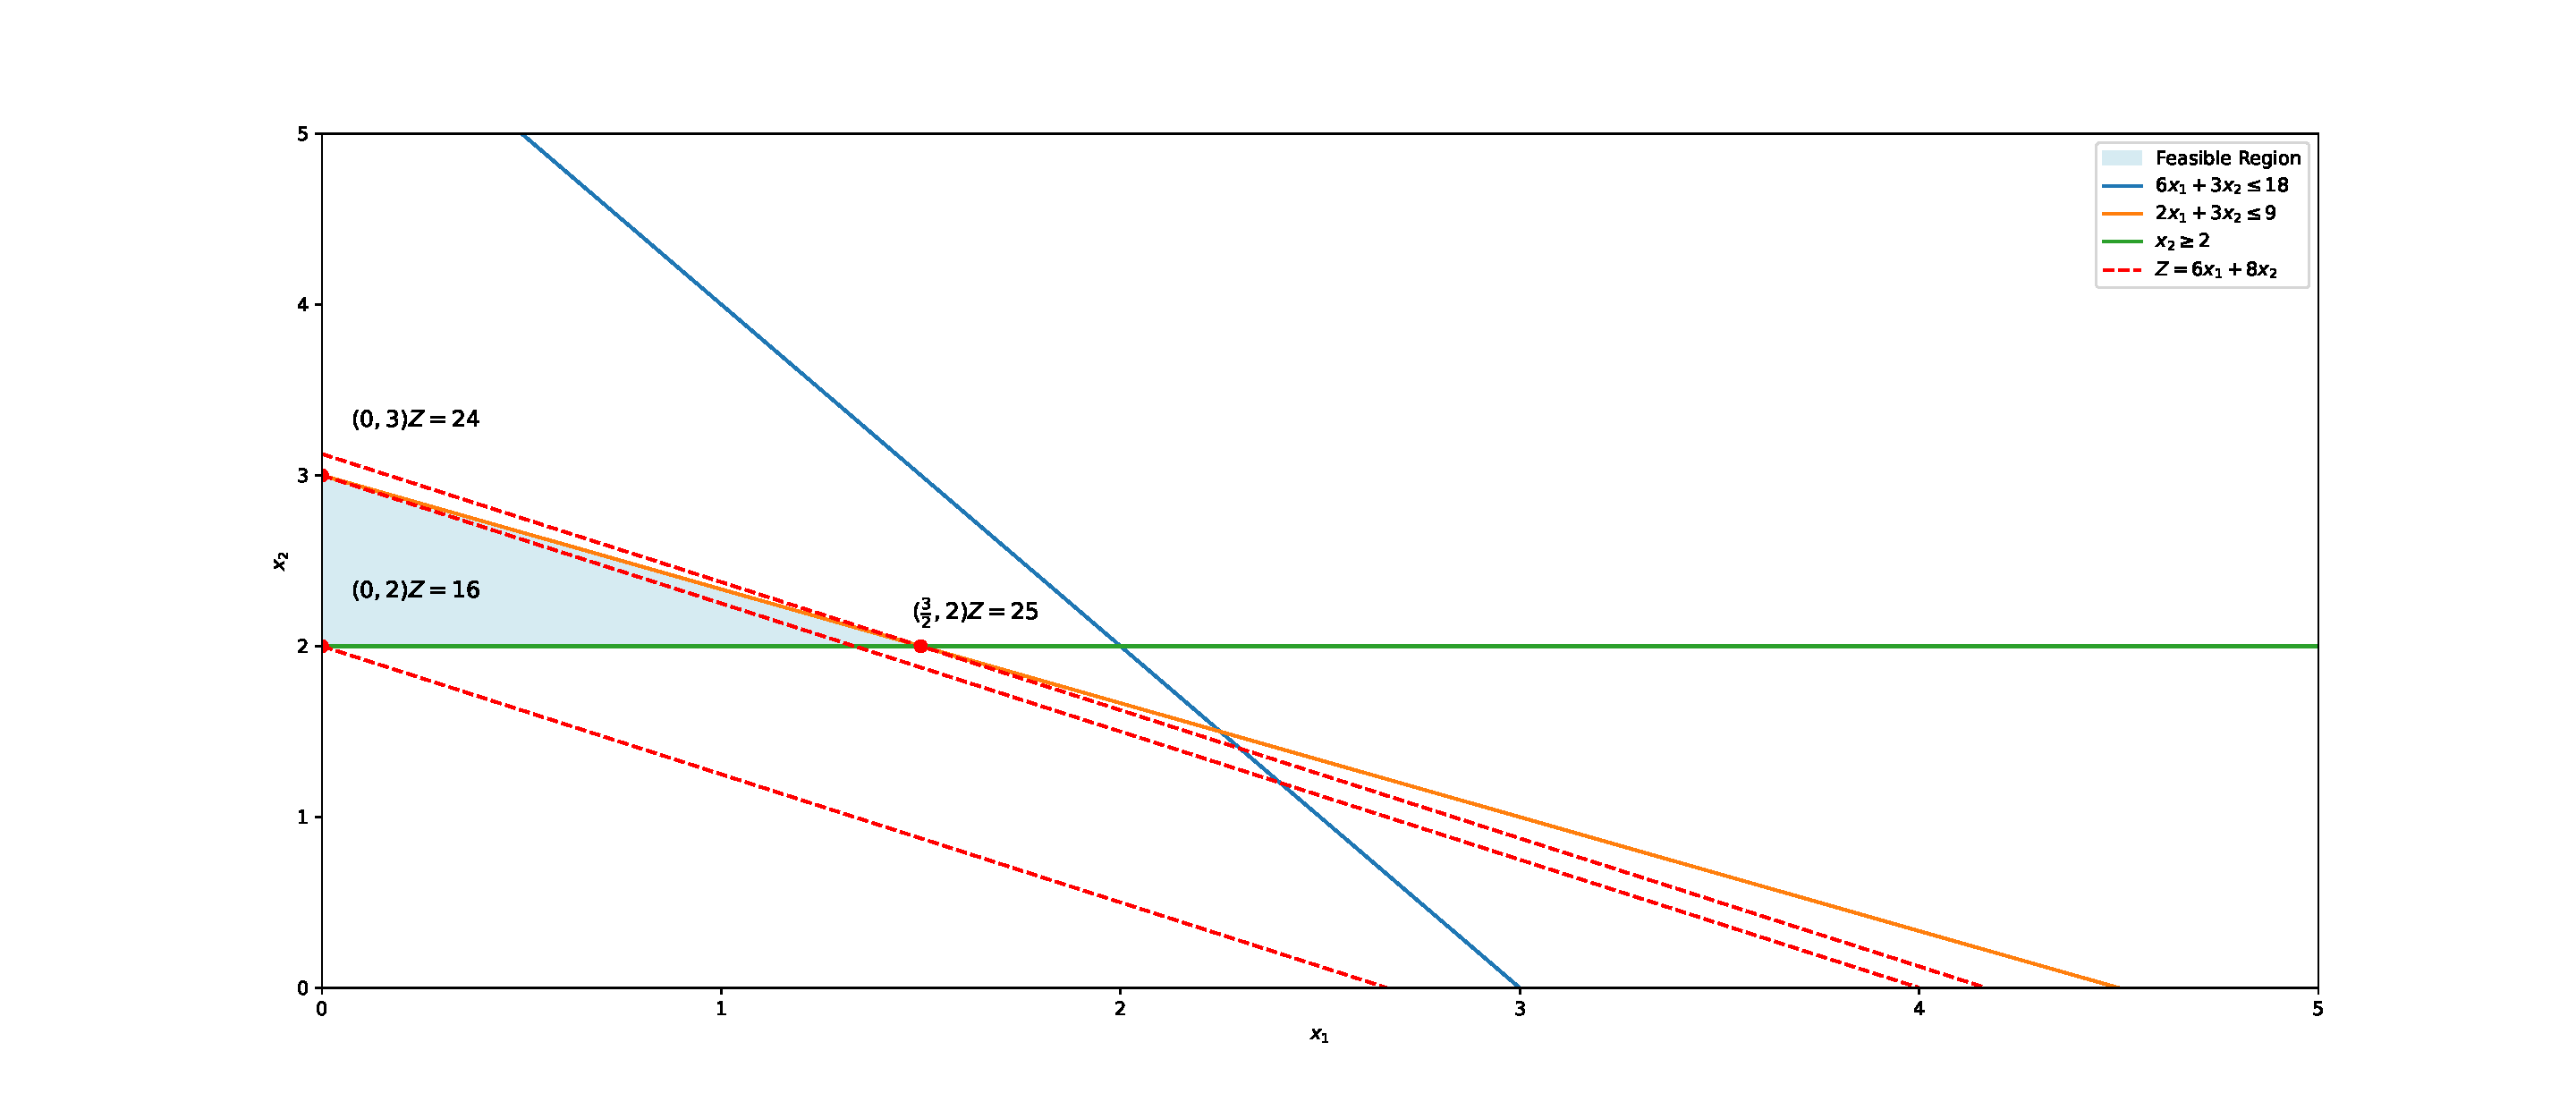
\includegraphics[width = \textwidth]{Exercice/PY/EX1/ex1.5.pdf}
\end{center}
\begin{center}
    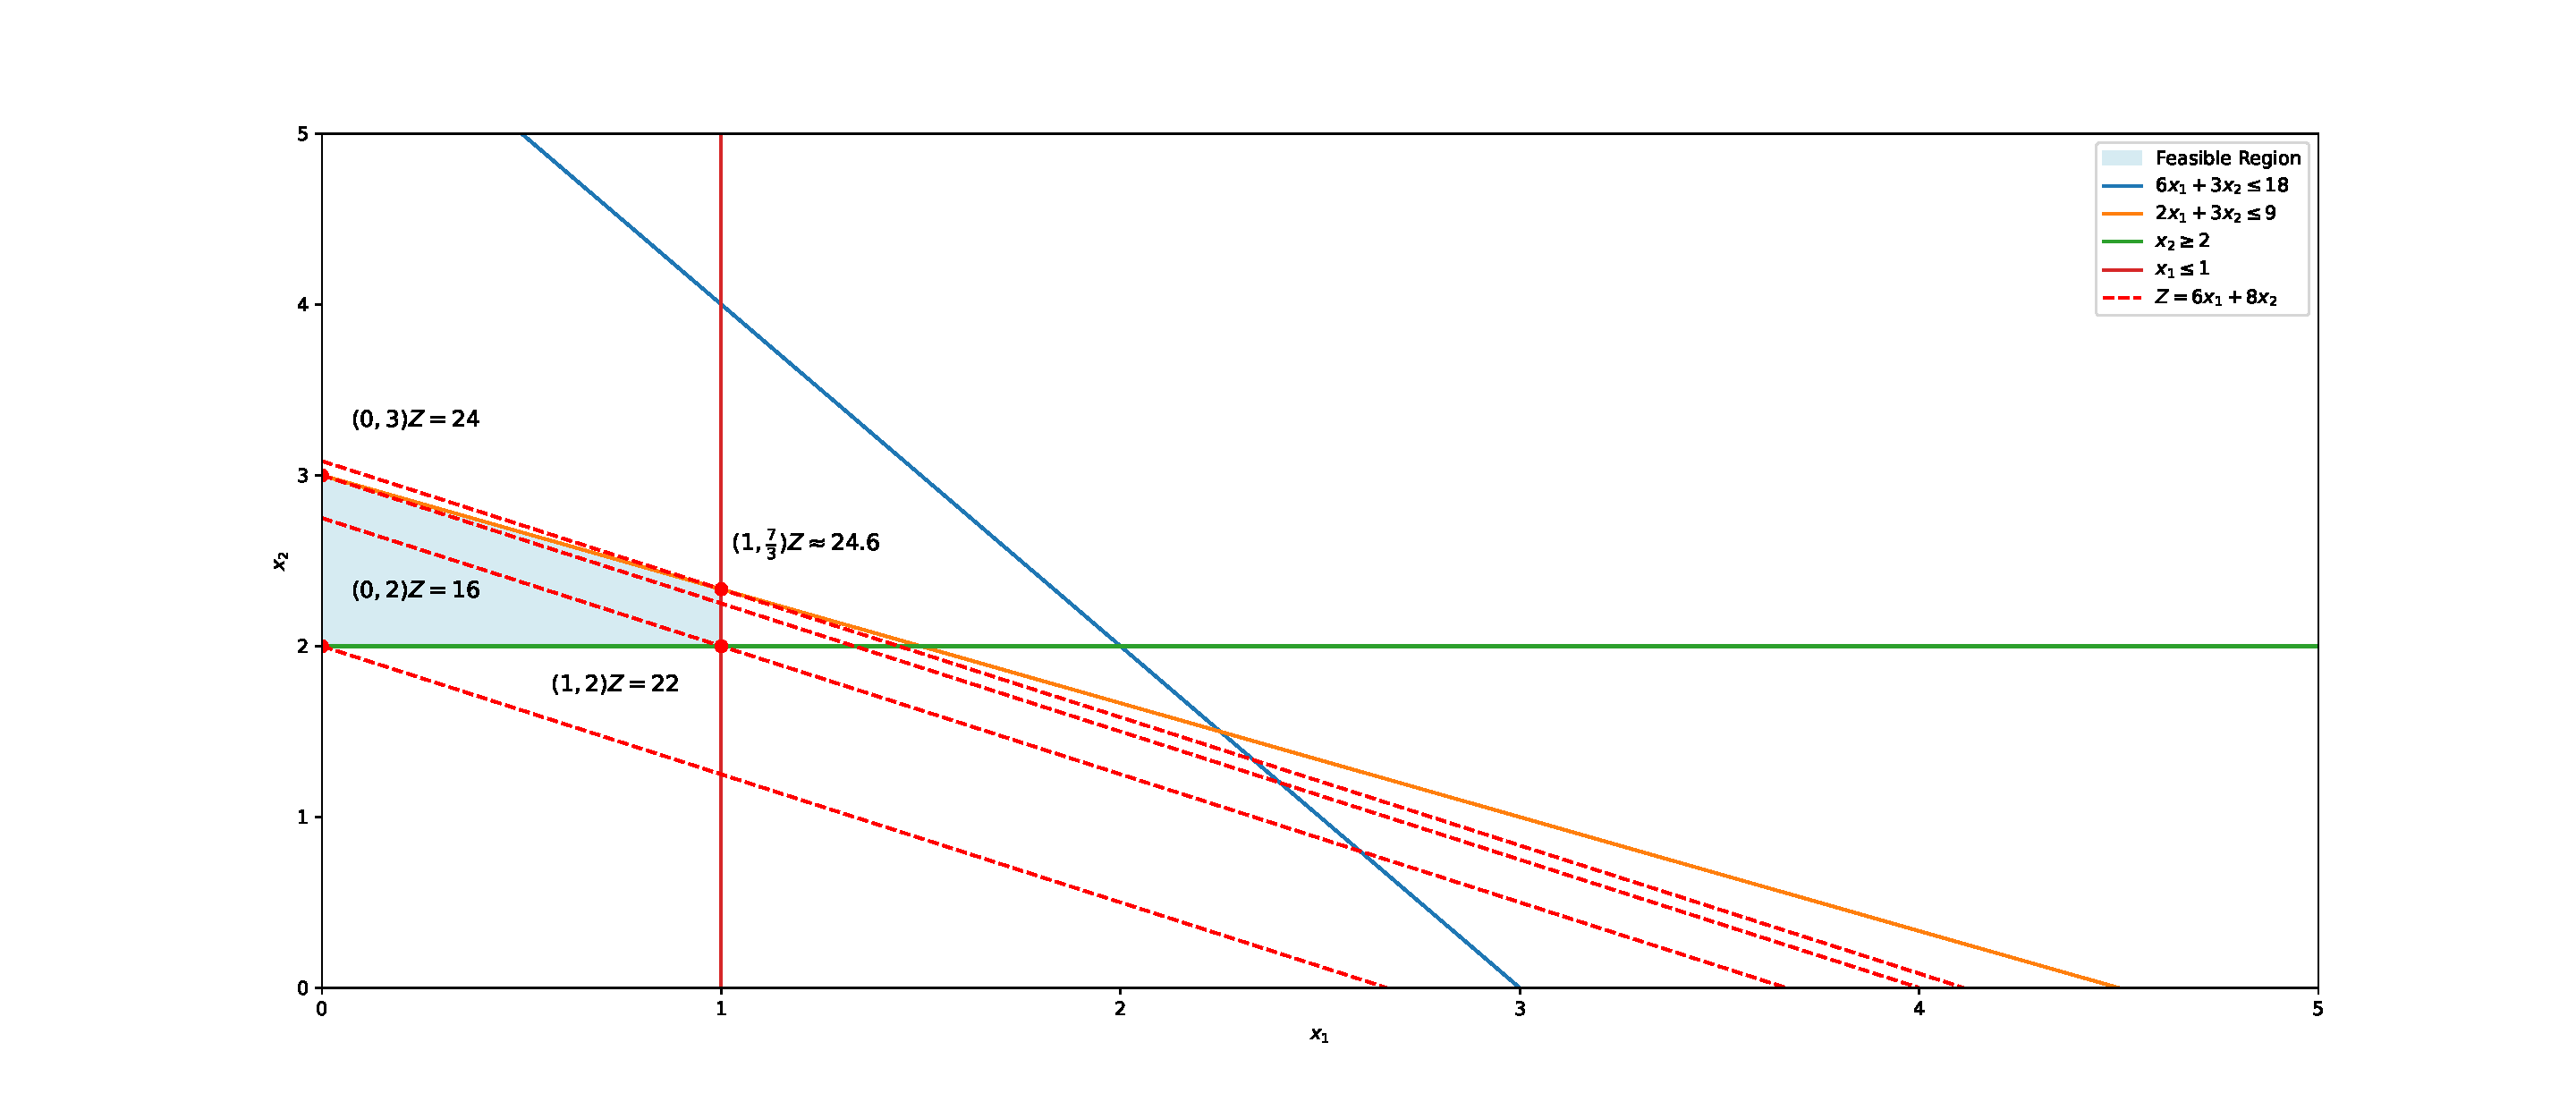
\includegraphics[width = \textwidth]{Exercice/PY/EX1/ex1.6.pdf}
\end{center}
\begin{center}
    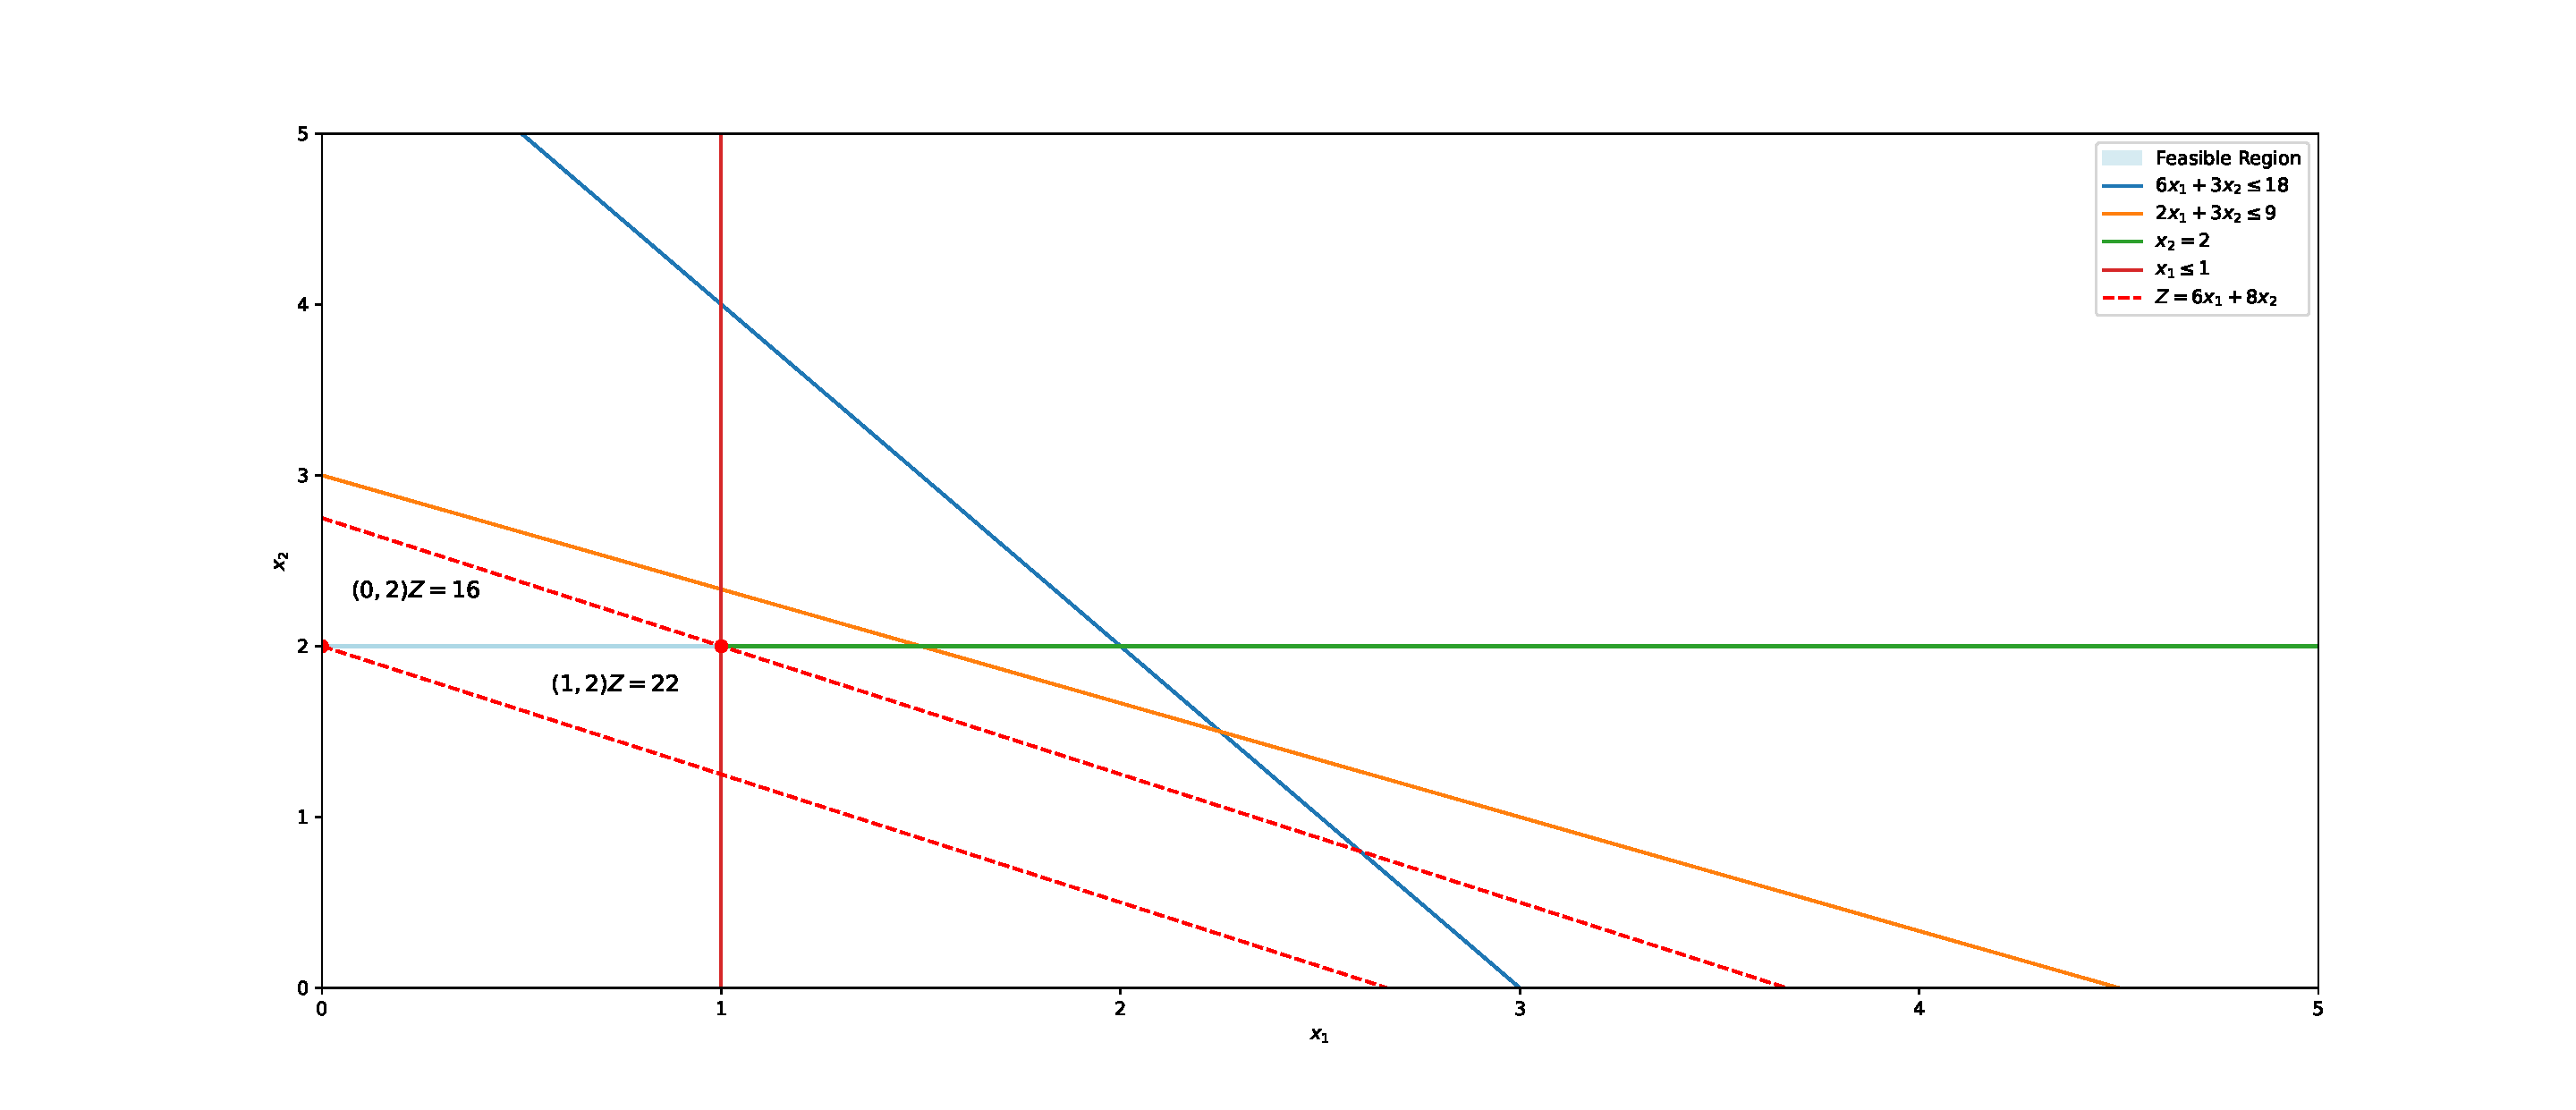
\includegraphics[width = \textwidth]{Exercice/PY/EX1/ex1.7.pdf}
\end{center}
\begin{center}
    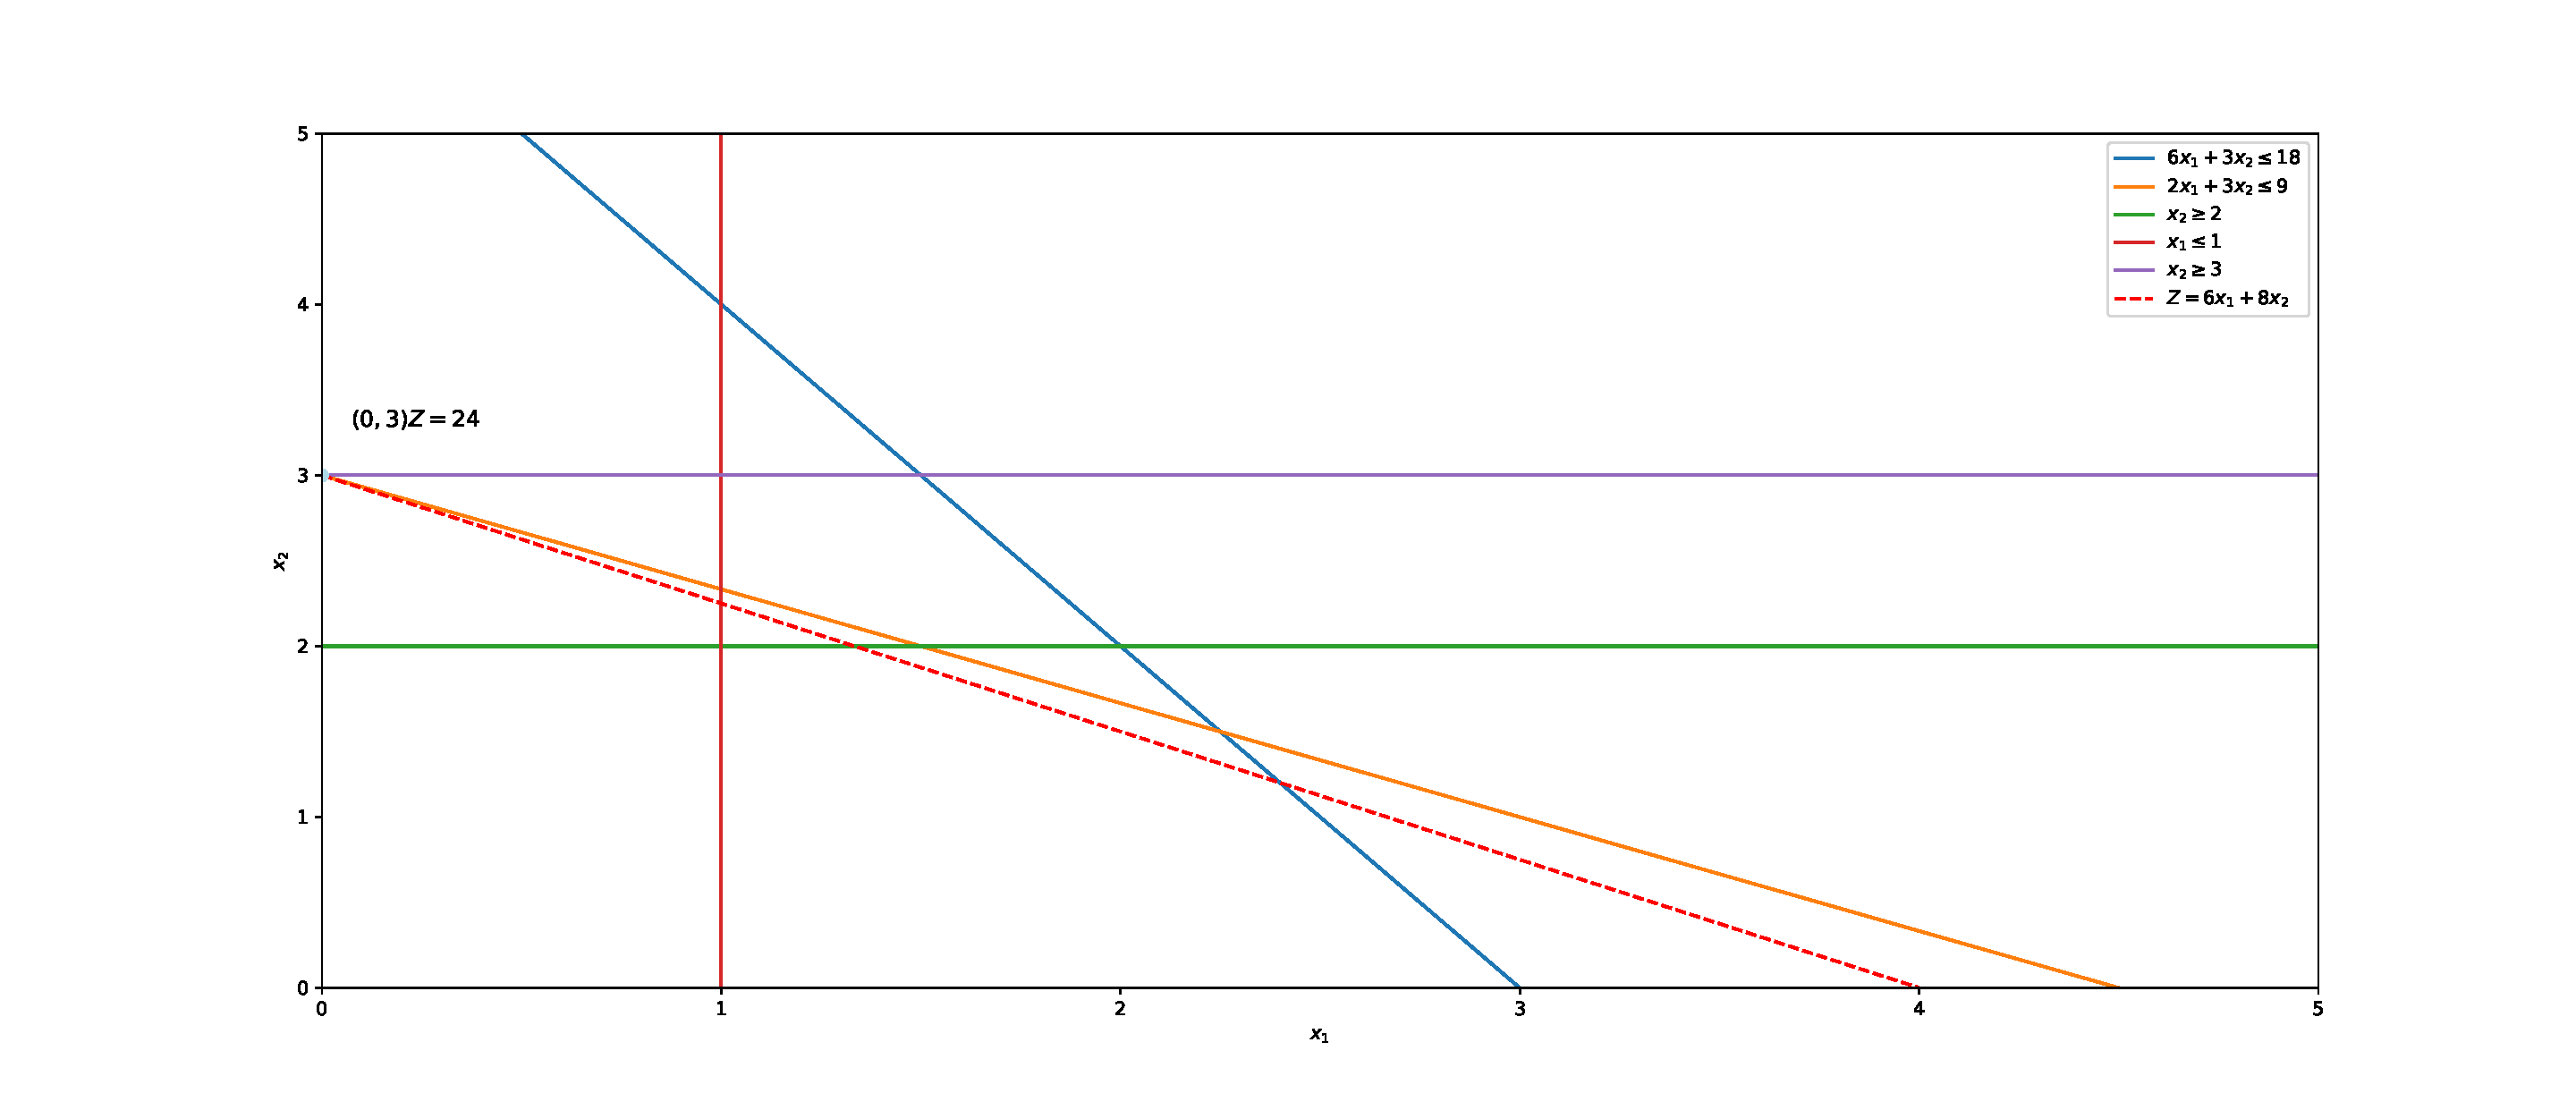
\includegraphics[width = \textwidth]{Exercice/PY/EX1/ex1.8.pdf}
\end{center}
\begin{center}
    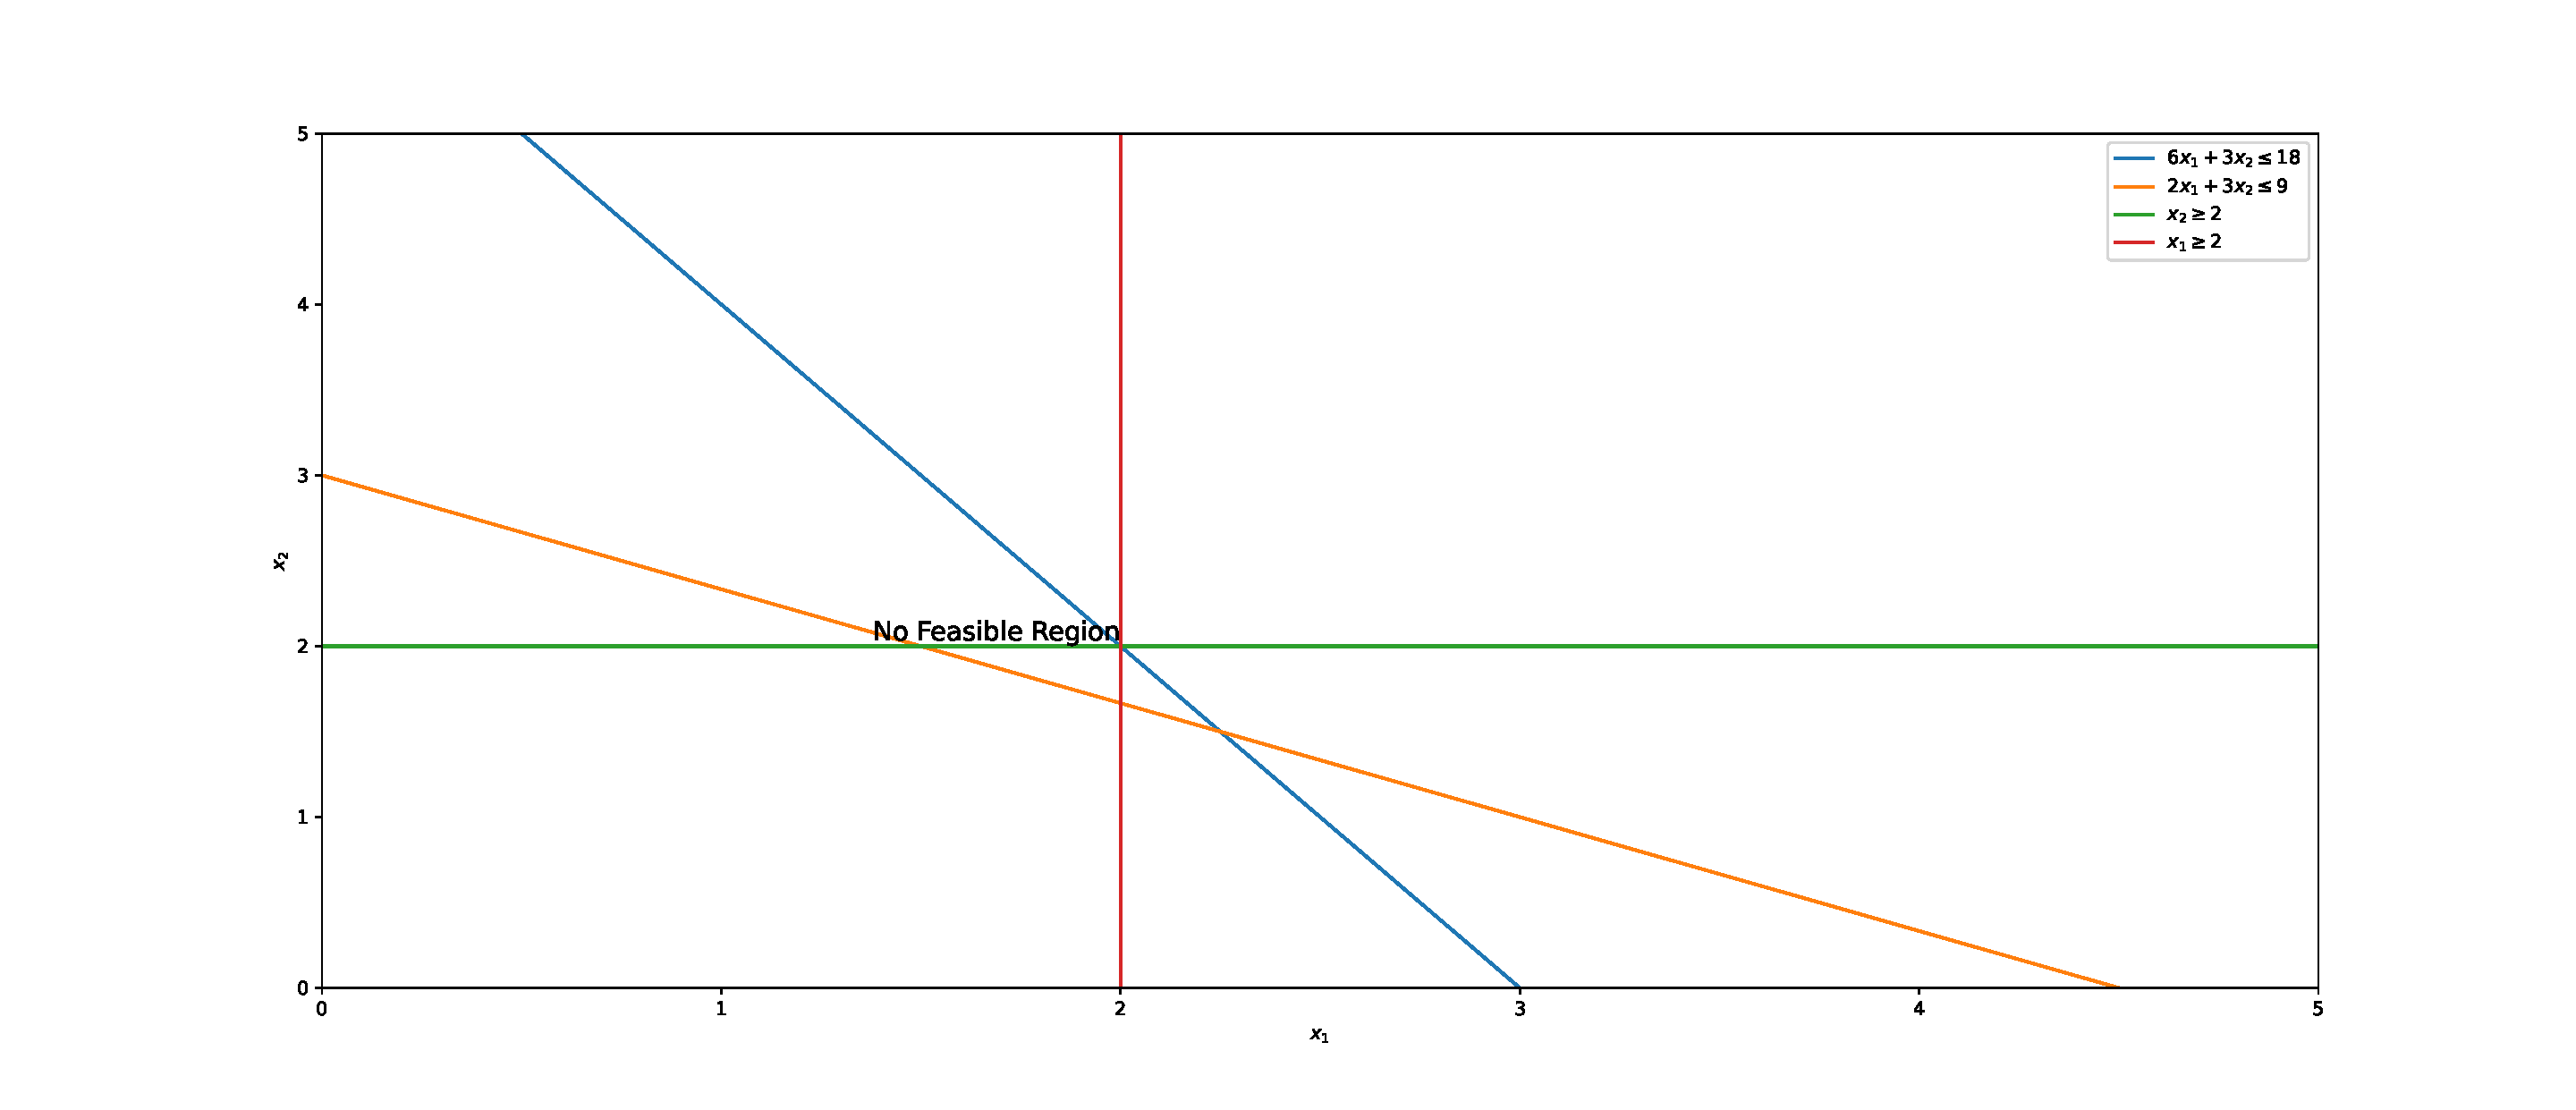
\includegraphics[width = \textwidth]{Exercice/PY/EX1/ex1.9.pdf}
\end{center}



